% =====================================================================
%  统一文档模板（全文唯一模板，不再中途切换版式）
%  类    ：ctexart / A4 / 12pt / Windows 中文字体
%  版心  ：四周 2.35cm，全文（含所有插图页）完全一致
%  标题  ：section / subsection 统一字号、字重与前后间距
%  图表  ：统一 caption 样式，图注在下、表注在上
%  页眉脚：全文统一，左侧文档名、右侧页码
%  插图  ：独立图 PDF 由 \reportgraphic 等比嵌入，不裁剪
% =====================================================================
\documentclass[UTF8,a4paper,12pt,fontset=windows]{ctexart}
\usepackage[margin=2.35cm,headsep=0.55cm,footskip=0.9cm]{geometry}
\usepackage{fancyhdr}
\usepackage{graphicx}
\usepackage{float}
\usepackage{booktabs}
\usepackage{tabularx}
\usepackage{longtable}
\usepackage{needspace}
\usepackage{array}
\usepackage{enumitem}
\usepackage{caption}
\usepackage{hyperref}
\usepackage{xcolor}
\usepackage{tikz}
\usetikzlibrary{calc,arrows.meta,fit,positioning}
% Ordinary UML actor for analysis sequence diagrams, as shown in the course.
% Keep the established black person strokes and proportions at 0.0275 cm
% per source SVG unit, without the business-worker circle or slash.
\tikzset{
  pics/analysis-actor/.style={code={
    \draw[draw=black,fill=white,line width=0.0605cm]
      (0,0.5225) circle[radius=0.1925cm];
    \draw[draw=black,line width=0.0605cm,line cap=butt]
      (0,0.33)--(0,-0.165)
      (-0.3575,0.1375)--(0.3575,0.1375)
      (0,-0.165)--(-0.3575,-0.66)
      (0,-0.165)--(0.3575,-0.66);
  }}
}

\hypersetup{colorlinks=true,linkcolor=black,urlcolor=black,citecolor=black}

% ---------- 标题样式（全文统一） ----------
\ctexset{
  section/format    = \Large\bfseries\raggedright,
  section/beforeskip= 2.2ex plus 1ex minus .2ex,
  section/afterskip = 1.4ex plus .3ex,
  subsection/format    = \large\bfseries\raggedright,
  subsection/beforeskip= 1.8ex plus .8ex minus .2ex,
  subsection/afterskip = 1.0ex plus .2ex,
}

% ---------- 段落与表格（全文统一） ----------
\setlength{\parindent}{2em}
\setlength{\parskip}{0.35em}
\renewcommand{\arraystretch}{1.25}
\newcolumntype{Y}{>{\raggedright\arraybackslash}X}
\newcolumntype{L}[1]{>{\raggedright\arraybackslash}p{#1}}
\newcolumntype{Z}{>{\raggedright\arraybackslash}p{11.6cm}}

% ---------- 图表标题（全文统一） ----------
\captionsetup{font=small,labelfont=bf,labelsep=space,skip=6pt}
\captionsetup[table]{position=top}

% ---------- 页眉页脚（全文统一） ----------
\pagestyle{fancy}
\setlength{\headheight}{14pt}
\fancyhf{}
\fancyhead[L]{\small 口腔诊所管理系统分析与设计报告}
\fancyhead[R]{\small\thepage}
\renewcommand{\headrulewidth}{0.4pt}
\fancypagestyle{plain}{%
  \fancyhf{}%
  \fancyhead[L]{\small 口腔诊所管理系统分析与设计报告}%
  \fancyhead[R]{\small\thepage}%
  \renewcommand{\headrulewidth}{0.4pt}%
}

% ---------- PDF 插图：宽、高只作为上限，保持原比例 ----------
\graphicspath{{figures/}}
\newcommand{\reportgraphic}[3]{%
  \includegraphics[width=#1,height=#2,keepaspectratio]{#3}}
\newcommand{\docgraphic}[1]{\reportgraphic{0.92\textwidth}{0.86\textheight}{#1}}
\newcommand{\figref}[1]{图~\ref{#1}}
\title{口腔诊所管理系统\\系统分析与设计报告}
\author{陈荣杰 \\ 信管 T2401 \\ 8305240320}
\date{2026 年 10 月 7 日}
\begin{document}
\begin{titlepage}
\centering
\vspace*{0.6cm}
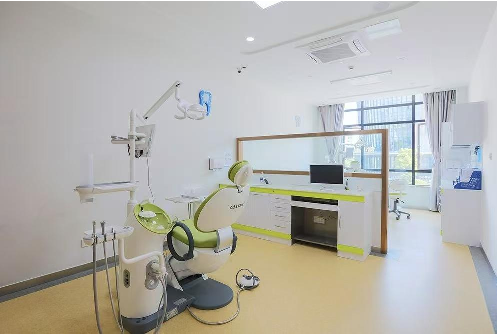
\includegraphics[width=0.92\textwidth]{cover.pdf}
\vspace{0.8cm}
{\zihao{2}\bfseries \mbox{口腔诊所管理系统}\par}
\vspace{0.35cm}
{\zihao{2}系统分析与设计报告\par}
\vspace{1.3cm}
\begin{tabular}{L{3.2cm}L{8.0cm}}
项目名称 & 口腔诊所管理系统 \\
姓名 & 陈荣杰 \\
学号 & 8305240320 \\
班级 & 信管 T2401 \\
日期 & 2026 年 10 月 7 日
\end{tabular}
\vfill
\end{titlepage}

\tableofcontents
\clearpage

\section{项目愿景}
\begin{table}[H]
\centering
\caption{愿景定义}
\begin{tabularx}{\textwidth}{L{3.2cm}Y}
\toprule
要素 & 定义 \\
\midrule
系统 & 口腔诊所管理系统 \\
目标组织 & 口腔诊所的前台、诊室、收费和合作技工协作流程 \\
老大 & 口腔诊所负责人 \\
目标 & 缩短患者首次受理到预约确认、收费完成和义齿订单交付的业务周期，提升记录可追溯性 \\
度量指标 & 预约确认周期中位数、预约兑现率、欠款回收率、义齿按期交付率、患者记录关联完整度 \\
\bottomrule
\end{tabularx}
\end{table}

以上线前连续 4 周的业务记录为基线，上线后按同一口径复核。验收目标为：预约确认周期中位数较基线下降 30\%，义齿订单按期交付率达到 90\% 以上，收费记录与患者、诊疗记录的关联完整度达到 99\% 以上。

\section{业务建模}
\subsection{业务用例}
业务用例以诊所为组织边界，患者、合作义齿技工所、支付机构和诊所负责人作为外部参与者。图 1 表示诊所向他们提供的业务结果，岗位之间的具体操作则由业务序列图说明。
\begin{table}[H]
\centering
\caption{业务参与者与业务价值}
\begin{tabularx}{\textwidth}{L{3.0cm}Y}
\toprule
参与者 & 需要获得或返回的业务结果 \\
\midrule
患者 & 获得连续的口腔诊疗服务，能够查询预约、诊疗和义齿交付进展。 \\
合作义齿技工所 & 接收修复要求，并返回接收、试戴、交货或返工状态。 \\
支付机构 & 接收支付请求，并返回成功、失败或待确认结果。 \\
诊所负责人 & 查看收费、欠款、订单周期和预约兑现等经营结果。 \\
\bottomrule
\end{tabularx}
\end{table}
\begin{figure}[H]\centering\docgraphic{01_business_usecase.pdf}\caption{口腔诊所业务用例图}\label{fig:business}\end{figure}

诊所对外提供的五类业务结果是连续的口腔诊疗、预约复诊、费用结算、可追踪的义齿交付和经营分析，涉及患者、支付机构、合作技工所及诊所负责人。同一名患者会参与多个业务环节，因此患者档案需作为统一的主数据维护，供各岗位共同使用，避免分别建档。

\subsection{现状业务序列}
接待时，患者先向前台提供资料。前台登记信息后，查询纸质档案或 Excel，再把资料转给医生、收费员或技工所。各岗位分别处理，交接通常依靠纸单或电话，消息往返顺序见图 2。

\begin{figure}[H]\centering\docgraphic{02_current_sequence.pdf}\caption{现状业务序列图}\label{fig:current-seq}\end{figure}

患者资料分散在纸面、Excel 和电话记录中。核对同一患者的预约、诊疗和收费情况时，需要分别查找各岗位的记录。

\subsection{改进后的业务序列}
改进后的流程由系统统一保存患者档案、预约、诊疗、收费和义齿加工信息，替代各岗位分散保管的记录。系统在业务序列中作为新的业务实体，与各岗位协作；医生和技工所根据同一张订单更新进度，消息顺序见图 3。

\begin{figure}[H]\centering\docgraphic{03_improved_sequence.pdf}\caption{改进后的业务序列图}\label{fig:improved-seq}\end{figure}

前台建档后，医生补充诊疗信息并生成义齿订单，技工所随后回报进度。系统保存接收、试戴、交货或返工状态，前台可直接查询订单，无需翻查聊天记录。收费与诊疗记录通过患者编号关联，便于核对。

\begin{table}[H]
\centering
\caption{现状到改进的业务映射}
\begin{tabularx}{\textwidth}{L{3.4cm}L{5.0cm}Y}
\toprule
现状断点 & 改进业务能力 & 验收结果 \\
\midrule
登记册、Excel 与收费单据分散 & 患者、预约、诊疗和收费使用统一患者编号 & 减少重复录入，可还原收费过程 \\
纸面日历缺少冲突状态 & 预约按医生、诊室、时间和状态查询 & 今日、明日和期间查询口径一致 \\
加工要求通过纸单或聊天传递 & 订单记录牙位、产品、颜色、附件、承诺日和状态 & 接收、试戴、交货和返工可追踪 \\
月底人工汇总 & 统计读取业务记录并保留样本量和异常数 & 指标可回到明细 \\
\bottomrule
\end{tabularx}
\end{table}

\section{系统需求建模}
\subsection{系统用例}
图 4 左侧为发起操作的岗位，包括前台、医生、收费员和诊所负责人；右侧为接收系统请求或反馈的外部参与者。患者接收预约或提醒，技工所接收义齿订单，支付服务处理支付请求。

左侧连线表示岗位发起系统功能，右侧连线表示系统与外部对象交互，位置用于提示交互方向。欠款查询、基础信息维护和经营统计由诊所内部岗位完成。

\begin{table}[H]
\centering
\caption{系统用例的发起与接收方向}
\begin{tabularx}{\textwidth}{L{2.5cm}L{4.8cm}Y}
\toprule
位置 & 参与者 & 交互说明 \\
\midrule
左侧发起者 & 前台接待、口腔医生、收费员、诊所负责人 & 发起登记、预约、诊疗订单、收费、欠款、基础信息和统计功能。 \\
右侧接收者 & 患者、合作义齿技工所、支付服务 & 接收预约或提醒、义齿订单和支付请求，并返回相应结果。 \\
\bottomrule
\end{tabularx}
\end{table}

\begin{table}[H]
\centering
\caption{功能需求清单}
\begin{tabularx}{\textwidth}{L{2.3cm}Y}
\toprule
功能域 & 可验收功能 \\
\midrule
基础信息 & 收费价目表、颜色定义、产品、员工、医院、订单类型、盒子颜色、单位和随单附件的配置。 \\
患者管理 & 患者登记、患者查询、期间登记查询、联系方式和重要提示维护。 \\
费用管理 & 收费录入、价目调用、支付结果记录、欠款查询和收费单追溯。 \\
预约管理 & 预约登记、医生/诊室/时间冲突检查、今日/明日/期间预约查询、确认/到诊/取消/爽约状态。 \\
订单录入 & 义齿订单、牙位、产品、颜色、数量、附件、技工所、承诺日期和状态。 \\
查询统计 & 试戴查询、已交货查询、订单提醒、预约兑现、收费欠款和订单周期统计。 \\
\bottomrule
\end{tabularx}
\end{table}

\begin{figure}[H]\centering\docgraphic{04_system_usecase.pdf}\caption{口腔诊所管理系统用例图}\label{fig:system-usecase}\end{figure}

系统功能分为面向患者的业务办理和诊所内部的日常管理。前者包括登记、预约、收费和订单录入，后者包括基础信息维护和查询统计。患者、合作技工所及支付服务不直接操作系统，图中由系统指向他们的连线表示发送预约、提醒、订单或支付请求。

\subsection{核心数据域}
患者、预约、诊疗记录、收费单、义齿订单及其状态、产品和欠款构成核心数据域。图 5 表示记录之间的数量关系，表 6 说明各组关系的业务含义。
\begin{figure}[H]
\centering
\resizebox{0.92\textwidth}{!}{%
\begin{tikzpicture}[
  x=1.2cm, y=1.42cm,
  concept/.style={draw, rectangle, minimum width=2.35cm, minimum height=0.82cm, inner sep=3pt, font=\normalsize},
  relation/.style={line width=0.55pt},
  multiplicity/.style={font=\normalsize}
]
  \node[concept] (patient) at (0,0) {患者};
  \node[concept] (appointment) at (-2.8,3.0) {预约};
  \node[concept] (medical) at (3.0,0) {诊疗记录};
  \node[concept] (order) at (6.3,0) {义齿订单};
  \node[concept] (bill) at (3.0,-3.0) {收费单};
  \node[concept] (debt) at (7.2,-3.0) {欠款};
  \node[concept] (status) at (9.7,3.0) {订单状态};
  \node[concept] (product) at (9.7,-2.0) {产品};

  \draw[relation] (patient.north east) -- (appointment.south);
  \node[multiplicity,above left=1pt] at ($(patient.north east)!0.16!(appointment.south)$) {1};
  \node[multiplicity,above right=1pt] at ($(patient.north east)!0.82!(appointment.south)$) {0..*};

  \draw[relation] (patient.east) -- (medical.west);
  \node[multiplicity,above=2pt] at ($(patient.east)!0.14!(medical.west)$) {1};
  \node[multiplicity,above=2pt] at ($(patient.east)!0.84!(medical.west)$) {0..*};

  \draw[relation] (patient.south east) -- (bill.west);
  \node[multiplicity,below left=1pt] at ($(patient.south east)!0.16!(bill.west)$) {1};
  \node[multiplicity,above right=1pt] at ($(patient.south east)!0.82!(bill.west)$) {0..*};

  \draw[relation] (medical.east) -- (order.west);
  \node[multiplicity,above=2pt] at ($(medical.east)!0.14!(order.west)$) {1};
  \node[multiplicity,above=2pt] at ($(medical.east)!0.84!(order.west)$) {0..*};

  \draw[relation] (bill.east) -- (debt.west);
  \node[multiplicity,below=5pt,xshift=-5pt] at ($(bill.east)!0.22!(debt.west)$) {1};
  \node[multiplicity,below=5pt,xshift=5pt] at ($(bill.east)!0.78!(debt.west)$) {0..1};

  \draw[relation] (order.north east) -- (status.south west);
  \node[multiplicity,above left=1pt] at ($(order.north east)!0.16!(status.south west)$) {1};
  \node[multiplicity,above right=1pt] at ($(order.north east)!0.82!(status.south west)$) {1..*};

  \draw[relation] (order.south east) -- (product.north west);
  \node[multiplicity,below left=1pt] at ($(order.south east)!0.18!(product.north west)$) {*};
  \node[multiplicity,below right=1pt] at ($(order.south east)!0.82!(product.north west)$) {1};
\end{tikzpicture}%
%
}
\caption{核心数据域关系图}
\label{fig:data-domain}
\end{figure}

\begin{table}[H]
\centering
\caption{数据关系及业务含义}
\begin{tabularx}{\textwidth}{L{4.8cm}Y}
\toprule
关系 & 业务含义 \\
\midrule
患者—预约、诊疗记录、收费单 & 一位患者可以有多次预约、诊疗记录和收费记录，患者编号用于串联历史。 \\
诊疗记录—义齿订单 & 一条诊疗记录可以产生多个修复订单，订单保留牙位、产品和承诺日期。 \\
义齿订单—订单状态、产品 & 每个订单至少有一条状态记录，并关联一个产品。 \\
收费单—欠款 & 一张收费单可以没有欠款，也可以对应一条欠款记录；欠款记录只对应一张收费单。 \\
\bottomrule
\end{tabularx}
\end{table}

患者编号将预约、诊疗和收费记录关联起来，支持一并查询，也便于检查重复建档、收费未关联诊疗或订单漏记状态等问题；欠款记录也须能追溯到对应收费单。没有对应诊疗记录的收费单缺少业务依据；义齿订单缺少状态记录，说明技工所回执尚未回填。将这些缺项纳入日常查询，负责人无需等到月底汇总才发现问题。

\section{用例规约}
\subsection{规约关系}
图 6 用矩形表示用例规约要素，以关系线连接相关部分，空心三角箭头表示扩展、包含和补充约束。

用例由主执行者发起，辅执行者在流程中提供协作。基本路径和扩展路径规定操作步骤，前置、后置条件分别限定流程开始与结束时的状态。字段列表列明业务数据，验收时还需核对业务规则、质量需求和设计约束。

\begin{figure}[H]\centering\docgraphic{06_usecase_spec.pdf}\caption{用例规约关系图}\label{fig:usecase-spec}\end{figure}

\begin{table}[H]
\centering
\caption{需求类别与规约要素映射}
\begin{tabularx}{\textwidth}{L{3.2cm}Y}
\toprule
需求类别 & 对应用例规约要素 \\
\midrule
功能需求 & 用例、路径、步骤、字段列表、业务规则 \\
质量需求 & 质量需求 \\
设计约束 & 设计约束 \\
\bottomrule
\end{tabularx}
\end{table}

\Needspace{7\baselineskip}
\subsection{UC-01 登记患者并预约诊疗}
\begin{longtable}{L{3.1cm}Z}
\caption{UC-01 用例规约}\label{tab:uc01}\\
\toprule 项目 & 内容 \\ \midrule
\endfirsthead
\toprule 项目 & 内容 \\ \midrule
\endhead
执行者 & 前台接待（主执行者）；患者（涉众） \\
前置条件 & 前台已登录；患者、医生、诊室和预约类型基础信息可用。 \\
后置条件 & 系统创建或更新患者档案，为预约生成唯一编号，并保存状态、操作者和时间。 \\
基本路径 & 1. 前台提交患者身份、联系方式和主诉。2. 系统检查患者记录。3. 前台确认档案。4. 前台提交医生、诊室、日期和时段。5. 系统检查冲突并反馈可用时段。6. 前台确认预约。7. 系统保存预约并反馈编号。 \\
扩展 & 无法确认同一患者时建立待核对档案；医生或诊室冲突时返回冲突原因；改约时保留原预约历史；保存失败时保留重试信息。 \\
字段列表 & 患者编号、姓名、电话、出生日期、主诉、重要提示；预约编号、患者编号、医生、诊室、日期时间、预约类型、状态、创建人。 \\
业务规则 & 同一医生或诊室同一时段不能有两个有效预约；状态为待确认、已确认、已到诊、已完成、已取消或爽约。 \\
质量需求 & 95\% 的标准预约查询在 2 秒内返回；熟悉流程的前台在 6 次操作内完成标准预约。 \\
设计约束 & 预约单沿用诊所负责人确认的字段和打印格式；预留短信或邮件提醒接口。 \\
\bottomrule
\end{longtable}

\Needspace{7\baselineskip}
\subsection{UC-02 录入收费并处理欠款}
\begin{longtable}{L{3.1cm}Z}
\caption{UC-02 用例规约}\label{tab:uc02}\\
\toprule 项目 & 内容 \\ \midrule
\endfirsthead
\toprule 项目 & 内容 \\ \midrule
\endhead
执行者 & 收费员（主执行者）；支付服务（辅助执行者） \\
前置条件 & 能找到患者及其诊疗项目或义齿订单；价目表有效。 \\
后置条件 & 收费单关联患者、诊疗或订单；系统保存支付结果和欠款余额。 \\
基本路径 & 收费员提交患者和项目标识；系统反馈待收费项目和价目；收费员确认数量、折扣和收款方式；系统计算应收、已收和欠款；系统请求支付；支付服务返回结果；系统保存收费单并反馈凭证。 \\
扩展 & 未找到项目时要求选择已有项目或交主管核对；支付失败保留失败原因；支付待确认时保留待确认状态；发现重复收费时拒绝提交。 \\
字段列表 & 单号、患者编号、诊疗项目或订单号、金额、折扣、应收、已收、欠款、支付方式、支付状态、经手人、时间。 \\
业务规则 & 应收=项目金额-合法折扣；欠款=应收-已收；支付状态为成功、失败、待确认或退款。 \\
质量需求 & 95\% 的标准收费查询在 3 秒内返回；收费与患者/诊疗/订单的关联完整度达到 99\% 以上。 \\
设计约束 & 支付卡号等敏感数据由支付服务保存；系统保留外部交易标识和结果。 \\
\bottomrule
\end{longtable}

\Needspace{7\baselineskip}
\subsection{UC-03 录入义齿订单并追踪交付}
\begin{longtable}{L{3.1cm}Z}
\caption{UC-03 用例规约}\label{tab:uc03}\\
\toprule 项目 & 内容 \\ \midrule
\endfirsthead
\toprule 项目 & 内容 \\ \midrule
\endhead
执行者 & 口腔医生（主执行者）；义齿技工所（辅助执行者）；前台接待（相关参与者） \\
前置条件 & 患者和诊疗记录存在；产品、颜色、单位、订单类型和附件可用。 \\
后置条件 & 订单有唯一编号；接收、试戴、质量确认、已交货或返工状态可追踪。 \\
基本路径 & 医生提交患者和修复要求；系统反馈基础信息；医生选择牙位、产品、颜色、数量、附件和承诺日期；系统校验并生成订单；医生确认发送；系统向技工所提供订单；技工所返回接收状态和预计完成时间；系统保存状态并形成提醒日期。 \\
扩展 & 基础信息缺失时转入维护；缺少牙位或附件时保持草稿；技工所拒收时标记待处理；试戴不合格时创建返工状态并保留历史。 \\
字段列表 & 订单号、患者编号、诊疗记录号、技工所、牙位、产品、颜色、数量、单位、附件、承诺日期、状态、发送时间、接收时间、交货时间。 \\
业务规则 & 状态为草稿、已发送、已接收、试戴、质量确认、已交货、返工或取消；已交货订单通过返工或更正记录修改。 \\
质量需求 & 订单状态变更在 1 分钟内可被前台和医生查询；订单关联完整度达到 99\% 以上。 \\
设计约束 & 订单支持打印或导出为技工所确认的格式；附件使用诊所批准的文件类型和大小限制。 \\
\bottomrule
\end{longtable}

\Needspace{7\baselineskip}
\subsection{UC-04 查询统计与订单提醒}
\begin{longtable}{L{3.1cm}Z}
\caption{UC-04 用例规约}\label{tab:uc04}\\
\toprule 项目 & 内容 \\ \midrule
\endfirsthead
\toprule 项目 & 内容 \\ \midrule
\endhead
执行者 & 诊所负责人（主执行者）；前台接待（相关参与者） \\
前置条件 & 患者、预约、收费或订单记录存在；查询期间合法。 \\
后置条件 & 系统反馈指标、样本量、明细入口和订单提醒状态。 \\
基本路径 & 负责人提交统计期间和业务类型；系统读取记录并计算预约兑现率、欠款回收率、订单按期交付率和记录关联完整度；系统反馈指标和明细；负责人选择待处理订单；系统反馈试戴、已交货和逾期提醒。 \\
扩展 & 数据量不足时显示样本量，不作趋势判断；记录无法关联患者或订单时标记数据质量异常；订单经其他渠道完成时，由负责人确认并保留原因。 \\
字段列表 & 查询条件、开始日期、结束日期、医生、业务类型、记录数、分子、分母、比率、中位时间、样本量和异常数。 \\
业务规则 & 待确认支付和未关闭订单不计入完成量；指标可追溯到原始记录；逾期按承诺日期和当前日期判断。 \\
质量需求 & 常用统计在 5 秒内反馈；导出结果与页面口径一致。 \\
设计约束 & 报表字段和格式由诊所负责人确认；按角色隐藏不必要的患者敏感信息。 \\
\bottomrule
\end{longtable}

\section{质量需求、追踪与实施}
\subsection{质量需求}
\begin{table}[H]
\centering
\caption{可验证质量需求}
\begin{tabularx}{\textwidth}{L{2.3cm}Y L{4.0cm}}
\toprule
质量属性 & 要求 & 验证方式 \\
\midrule
性能 & 患者、预约和收费查询 95\% 在 3 秒内返回；统计在 5 秒内返回 & 代表性数据量压测 \\
业务效率 & 预约确认周期中位数较基线下降 30\% & 上线前后同口径抽样 \\
一致性 & 同一医生/诊室时段不产生两个有效预约；订单状态不得无原因倒退 & 并发预约和状态机测试 \\
安全性 & 角色限制患者、收费和统计数据范围；敏感支付数据不进入系统 & 权限矩阵和字段审计 \\
可追溯性 & 关键修改保存操作者、时间、原值、新值和原因 & 抽样回放患者、收费和订单 \\
可恢复性 & 每日备份并完成恢复演练 & 备份检查和恢复记录 \\
\bottomrule
\end{tabularx}
\end{table}

\subsection{愿景到需求的追踪}
\begin{table}[H]
\centering
\caption{愿景、业务过程与系统用例追踪}
\begin{tabularx}{\textwidth}{L{3.4cm}L{4.5cm}L{1.4cm}Y}
\toprule
愿景结果 & 业务过程 & 用例 & 关键数据 \\
\midrule
缩短预约确认周期 & 登记、查询、冲突检查、确认 & UC-01 & 患者、预约、医生、诊室、状态 \\
明确收费来源与欠款计算依据 & 项目选择、收费、支付、结清 & UC-02 & 价目、收费单、支付状态、欠款 \\
提高义齿按期交付率 & 创建、发送、接收、试戴、交货、返工 & UC-03 & 订单、牙位、产品、颜色、附件、承诺日期 \\
支持负责人判断经营结果 & 统计、明细追踪、订单提醒 & UC-04 & 预约、收费、订单、样本量、异常 \\
\bottomrule
\end{tabularx}
\end{table}

\subsection{实施与验收}
\begin{table}[H]
\centering
\caption{实施阶段与验收场景}
\begin{tabularx}{\textwidth}{L{2.3cm}Y Y}
\toprule
阶段 & 实施重点 & 验收场景 \\
\midrule
主数据 & 清理重复患者档案，确认价目、产品、颜色、员工、医生、诊室和技工所 & 字段口径和基线样本经负责人确认 \\
患者与预约 & 登记、查询、今日/明日/期间预约和状态 & 同一医生同一时段冲突被拒绝，改约历史可回放 \\
收费与欠款 & 收费录入、支付结果、欠款查询和收费追溯 & 支付失败或待确认时欠款不被清零 \\
义齿订单 & 订单录入、附件、技工所状态、试戴和已交货查询 & 订单从发送到交货或返工完整回放 \\
统计与提醒 & 指标、明细追踪、订单提醒和导出 & 指标可回到明细，异常记录单独显示 \\
\bottomrule
\end{tabularx}
\end{table}

\clearpage
\section{分析类模型}
\AddToHook{env/tabularx/begin}{\linespread{1.08}\selectfont}
\subsection{分析边界与责任划分}
本章从前文四个用例继续展开。课程材料第 280 页进入分析建模，第 287--288 页说明边界类、控制类和实体类，第 313--332 页讨论分析序列图及责任分配；第 398--403 页说明关系数据库映射。这里沿用这条顺序：先确定对象负责什么，再画对象间的调用，最后设计表结构。

分析类图中的矩形按名称、属性和操作分栏。实线表示关联，端点数字表示多重性；实心菱形位于整体端，表示组成对象归整体管理。属性前的“/”表示派生值。分析阶段不把主键、外键或数据库访问操作加到业务实体中。

\begin{table}[H]
\centering\caption{用例与边界、控制、实体的对应关系}
\small
\begin{tabularx}{\textwidth}{L{1.3cm}L{3.3cm}L{3.4cm}Y}
\toprule
用例 & 边界类 & 控制类 & 主要实体类\\\midrule
UC-01 & 前台接口、消息服务接口 & 登记预约控制 & 患者、预约、医生、诊室、预约变更\\
UC-02 & 收费接口、支付服务接口 & 录入收费控制 & 诊疗、收费单、收费明细、收费项目、支付、欠款\\
UC-03 & 医生接口、技工所接口 & 录入义齿订单控制 & 诊疗、义齿订单、产品、技工所、订单牙位、订单进展、提醒\\
UC-04 & 负责人接口、前台接口、消息服务接口 & 查询统计与提醒控制 & 预约、收费单、义齿订单、提醒\\
维护与诊疗 & 管理接口、医生接口 & 基础信息维护控制、录入诊疗控制 & 医院诊所、基础选项、员工岗位、价目、产品、诊疗\\
\bottomrule
\end{tabularx}
\end{table}

前台接口等人机边界接收输入并显示结果；支付服务接口、技工所接口和消息服务接口适配外部交互。控制类按用例协调对象，不包揽计价、欠款计算和订单阶段判断。后面序列图中的类名均沿用本表；名字前的冒号表示该类的一个对象。患者查询按患者档案及登记日期检索，基础信息维护和录入诊疗为前文功能清单中的配套用例，复用相同实体。

\clearpage
\subsection{患者、预约与诊疗}
患者负责核对身份，预约负责确认时段及改变预约阶段，诊疗保存医生实际完成的诊疗内容。医生和诊室是预约需要占用的资源，冲突检查要同时考虑两者。这里的“医生”是员工承担的业务角色，数据库阶段仍引用员工表，不另造一套人员档案。

\begin{figure}[H]\centering
\reportgraphic{\textwidth}{0.72\textheight}{07_classes_appointment.pdf}
\caption{患者、预约与诊疗分析类图}\label{fig:analysis-appointment}
\end{figure}

一位患者可以有多次预约和诊疗。一次预约最多对应一次诊疗，现场到诊可以没有预约。改约或取消保留原时段、原阶段、原因、操作人和发生时间。

预约时段包含开始时刻，不包含结束时刻，前一预约结束时可接下一预约。“新开始早于旧结束，且新结束晚于旧开始”表示重叠。已取消和爽约记录不占用未来时段。

\clearpage
\subsection{收费、支付与欠款}
收费单统管自己的收费明细和支付尝试。明细保存开单时采用的名称、单位与单价，后续调整价目不会改变已开单据。支付对象确认外部交易结果；收费单据此计算有效已收，欠款对象跟踪未结清款项。

\begin{figure}[H]\centering
\reportgraphic{\textwidth}{0.72\textheight}{08_classes_billing.pdf}
\caption{收费、支付与欠款分析类图}\label{fig:analysis-billing}
\end{figure}

应收等于明细金额之和减去整单合法折扣。已收只累计成功的收款，扣除成功退款；失败和待确认支付不改变已收。欠款等于应收减有效已收，不能用“收到回调”代替“支付成功”。

每张收费单可以多次尝试支付或分次收款。首次欠款时建立欠款对象，结清后保留结清时间；从未发生欠款的收费单可以没有欠款对象。

\clearpage
\subsection{义齿订单与交付协作}
义齿订单负责校验修复要求、接受合法回执和决定当前阶段，订单进展负责留存每次变化。一个订单只选用一种产品，可以包含多个牙位；不同产品分开建立订单，便于分别约定交期和返工。订单附件是订单的组成部分，文件名、格式和存储位置在数据库设计中展开。

\begin{figure}[H]\centering
\reportgraphic{\textwidth}{0.72\textheight}{09_classes_order.pdf}
\caption{义齿订单、进展与提醒分析类图}\label{fig:analysis-order}
\end{figure}

订单至少保留一条进展，第一条记录草稿建立。技工所回执必须指向已有订单，来源与事件号用于识别重复通知。试戴不合格时追加返工进展，保留原来的试戴结果；已交货订单不能直接改回“已接收”。

\clearpage
预约阶段、支付结果和订单阶段都有明确的业务含义，因此在模型中保留。它们的改变由实体操作完成，控制类不能任意修改这些属性。类图沿用课程的三栏矩形、可见性符号和操作签名；返回类型 Patient、Bill、OrderCopy 等分别表示患者、收费单和订单副本，Metric 表示带样本量的指标结果。图中未强加继承关系，员工的多个岗位以角色关联表达。

\begin{table}[H]\centering\caption{关键操作的责任归属}
\small
\begin{tabularx}{\textwidth}{L{3.0cm}L{4.4cm}Y}
\toprule
对象 & 对外操作 & 负责判断的业务规则\\\midrule
预约 & 确认、改约、取消、登记到诊、汇总履约 & 医生与诊室的时段占用、有效阶段及预约兑现口径\\
收费单 & 拟定、计算应收、应用支付结果、汇总回收 & 价格快照、合法折扣、有效已收、欠款和回收口径\\
支付 & 登记尝试、确认结果 & 请求是否重复、结果能否迁移、成功金额是否已计入\\
义齿订单 & 保存草稿、发送、受理回执、登记试戴、确认交货、申请返工 & 必填修复要求、阶段迁移、重复回执和交付口径\\
提醒 & 排定、判断到期、确认发送 & 计划时间、收件人及重复发送限制\\
\bottomrule\end{tabularx}
\end{table}

\subsection{功能覆盖核对}
\begin{table}[H]\centering\caption{项目功能与模型覆盖}
\small\begin{tabularx}{\textwidth}{L{2.6cm}L{6.1cm}Y}
\toprule 功能域 & 对象与持久化数据 & 查询或处理结果\\\midrule
基础信息 & 医院诊所、员工岗位、产品、价目、分类选项 & 颜色、盒色、单位、订单类型及附件配置可维护、可停用\\
患者与诊疗 & 患者、诊疗；登记时间、接诊医生和主诉 & 按身份、电话、登记期间查患者，回看诊疗历史\\
预约 & 预约、预约变更、医生与诊室关联 & 今日、明日、期间查询，冲突检查和改约留痕\\
费用 & 收费明细、支付、欠款 & 项目计价、收款与退款、欠款查询及单据追溯\\
义齿订单 & 产品、牙位、颜色、附件、进展、交期 & 试戴、已交货、返工和逾期查询\\
统计与提醒 & 业务记录汇总、预约或订单提醒 & 指标、样本、异常明细、通知计划及发送结果\\
\bottomrule\end{tabularx}\end{table}

\clearpage
\section{分析序列模型}
\subsection{UC-01 登记患者并预约诊疗}
前台作为外部执行者发起调用，其余参与对象是软件内部对象。执行者采用课件中的普通人形符号。软件对象的侧边竖线圆表示边界类，带开放箭头圆表示控制类，底线圆表示实体类。同步调用采用实线和直边实心三角箭头，返回采用虚线和开放箭头，细长矩形表示执行片段。消息箭头落在执行条边缘，人物、对象和连线采用统一的细黑线。

图中从前台提交要求开始，省略窗口打开等操作。预约对象在提交时形成，确认前不占用有效预约名额；身份未核对清楚时先返回待核对结果，不强行合并患者档案。

\begin{figure}[H]\centering
\reportgraphic{\textwidth}{0.70\textheight}{10_sequence_appointment.pdf}
\caption{UC-01 登记与预约分析序列图}\label{fig:seq-appointment}
\end{figure}

\clearpage
\subsection{UC-02 录入收费并处理欠款}
收费单、明细和待确认支付先在本地保存，随后才向支付服务发起请求。这使超时后仍能按原请求号核对结果。下图展开基本路径；守卫条件和图下说明补足成功、失败、待确认三种分支。

\begin{figure}[H]\centering
\reportgraphic{\textwidth}{0.80\textheight}{11_sequence_billing.pdf}
\caption{UC-02 收费、支付与欠款分析序列图}\label{fig:seq-billing}
\end{figure}

\clearpage
\subsection{UC-03 录入义齿订单并追踪交付}
\subsubsection{医生建立并发送订单}
诊疗对象先确认业务依据，义齿订单再核对产品、牙位、数量、颜色和必要附件。发送订单与技工所接受订单是两个结果，不能把一次发送成功当作技工所已经开始加工。

\begin{figure}[H]\centering
\reportgraphic{\textwidth}{0.80\textheight}{12_sequence_order_send.pdf}
\caption{UC-03 订单建立与发送分析序列图}\label{fig:seq-order-send}
\end{figure}

\clearpage
\subsubsection{技工所回执与进展追踪}
本图承接\figref{fig:seq-order-send} 的订单号，展开稍后到达的回执。技工所接口核对来源和报文格式，订单对象判断事件是否重复、阶段变化是否合法。只有处理成功后才确认回执，失败时保留重试或核对入口。

\begin{figure}[H]\centering
\reportgraphic{\textwidth}{0.80\textheight}{13_sequence_order_receipt.pdf}
\caption{UC-03 技工所回执分析序列图}\label{fig:seq-order-receipt}
\end{figure}

\clearpage
\subsection{UC-04 查询统计与订单提醒}
控制类向相应实体请求按统一期间汇总，不逐字段取出数据后自行判断业务含义。预约负责兑现口径，收费单负责欠款回收口径，义齿订单负责交期口径。返回结果都带分子、分母、样本量及异常明细，便于负责人核对。

\begin{figure}[H]\centering
\reportgraphic{\textwidth}{0.80\textheight}{14_sequence_statistics.pdf}
\caption{UC-04 统计与待处理订单分析序列图}\label{fig:seq-statistics}
\end{figure}

\clearpage
\section{数据库逻辑设计}
\subsection{从分析类到关系表}
课程在关系数据库部分区分类、属性和对象与表、列和行的对应关系，并把一对多关联的外键放到多的一端。本设计采用关系数据库逻辑模型，字段类型暂用通用 SQL 名称，具体数据库选型留到实现阶段。

数据库图参考 Shopify 和 Quickbooks 的 ERD：用表框逐行列出字段、键和外键目标，以业务分区组织主表、明细、支付与历史记录。下图先给出完整关系，再分别展开预约、费用和义齿业务。全库共 20 张表、44 个外键，覆盖基础资料、患者、诊疗、预约、收费、订单及通知；统计直接使用这些业务记录。

\begin{table}[H]\centering\caption{分析对象到关系表的映射}
\small\begin{tabularx}{\textwidth}{L{3.0cm}L{5.4cm}Y}
\toprule
分析对象 & 关系表 & 映射理由\\\midrule
患者、医生、诊室 & patient、employee、clinic\_room & 医生以员工角色参与，患者有独立档案\\
基础信息与员工岗位 & clinic、basic\_option、employee\_role & 诊所资料、分类选项与员工兼岗分别维护\\
预约、预约变更、诊疗 & appointment、appointment\_event、encounter & 当前安排与变更历史分开，诊疗可选关联预约\\
收费单、收费明细、收费项目 & bill、bill\_line、price\_item & 明细引用价目并保留成交快照\\
支付、欠款 & payment、bill；欠款查询视图 & 保存每次支付尝试，欠款按有效收款计算，催收日期归属收费单\\
产品、技工所、义齿订单 & product、dental\_lab、dental\_order & 订单引用一个产品和一家技工所\\
牙位、进展、附件、提醒 & order\_tooth、order\_event、order\_attachment、reminder & 多值结构拆开保存，避免逗号拼接牙位或覆盖历史\\
\bottomrule\end{tabularx}\end{table}

图中 PK 为主键，FK 为外键，UK 为唯一约束，问号表示允许空值。UK* 表示联合唯一约束，组合范围在后文列出。每个字段单列一行，并在右侧写明外键引用的表；连线箭头从外键所在表指向被引用表。同一对表的多个外键合并为一条连线，各字段的具体目标仍逐一保留，表\ref{tab:foreign-keys} 列出完整清单。

订单牙位与员工岗位使用复合主键，其余表使用不带业务含义的 id 作为主键，业务编号另设唯一约束。医生、诊室等对象关联转成外键；边界类和控制类不直接转成表。欠款是收费单的派生业务对象，数据库通过查询视图计算余额，不再单设欠款表。形成时间、到期日、结清时间和催收备注保存在收费单中。

\clearpage
\subsection{完整数据库设计图}
\figref{fig:erd-overview} 将 20 张表放在同一张图中。患者、预约、诊疗、收费单和义齿订单构成业务主链；员工、诊室、价目和产品提供基础资料，变更、支付尝试、回执、附件和提醒保留处理过程。颜色用于区分业务分区，字段名称、类型和关系均保留为矢量内容。

\begin{figure}[H]\centering
\reportgraphic{\textwidth}{0.68\textheight}{15_erd_overview.pdf}
\caption{口腔诊所完整数据库设计图（20 张表）}\label{fig:erd-overview}
\end{figure}

全图以独立矢量 PDF 嵌入报告，页面中按比例显示，放大后可以逐字段查看。后三张局部图用于阅读密集区域，重复出现的引用表仅列主键，不增加实际表数。

预约除了起止时刻，还保存创建、确认、到诊、完成及取消时刻，用于核对确认周期和兑现结果。收费单保存折扣原因及催收信息；支付保存请求、结果、核对时间和失败原因，支持分次收款、超时核对与退款。订单保留发送、接收、试戴和交货时刻，进展表保留事件来源与事件号，避免只凭当前阶段倒推业务过程。

基础选项集中维护岗位、单位、颜色、盒色、订单类型、预约类型、支付方式、通知渠道和附件类型。相同选项表可以被多个业务字段引用，但业务操作必须核对其类别。例如，\texttt{role\_id} 只能引用岗位类别，不能引用颜色或单位。

\clearpage
\subsection{患者、预约与诊疗 ERD}
患者保存登记时间和经办人，支持期间登记查询。预约保存主诉、开始与结束时间，变更表保存变更前后值。诊疗可以没有预约，但必须属于一个患者并由一名医生完成。手机号可以多人共用，不能强制唯一。

\begin{figure}[H]\centering
\reportgraphic{\textwidth}{0.74\textheight}{16_erd_appointments.pdf}
\caption{患者、预约与诊疗数据库设计图}\label{fig:erd-appointment}
\end{figure}

\clearpage
\subsection{收费、支付与欠款 ERD}
收费单通过诊疗关联患者；明细可以关联同次诊疗下的义齿订单，并保存开单时采用的项目名称、单位、数量和单价。支付表同时记录收款、退款和未成功的尝试，退款通过 \texttt{refund\_of\_id} 回到原成功收款。

\begin{figure}[H]\centering
\reportgraphic{\textwidth}{0.70\textheight}{17_erd_billing.pdf}
\caption{收费、支付与欠款数据库设计图}\label{fig:erd-billing}
\end{figure}

欠款查询先分别按收费单汇总明细和有效支付，再将两个汇总结果关联，防止明细与支付直接连接造成金额重复。应收为明细数量乘成交单价、扣除行折扣和整单折扣；有效已收为成功收款减成功退款；欠款余额为两者之差。失败、待确认或已作废单据不计入已收或有效欠款。

\texttt{debt\_opened\_at} 记录首次形成欠款的时刻，\texttt{due\_date} 记录约定到期日，\texttt{settled\_at} 记录最近一次结清时刻。退款使欠款重新产生时清除结清标记，并保留原支付记录。查询期初欠款时按截止时刻重算历史收付，不能只读取今天的结清标记。

\clearpage
\subsection{义齿订单与进展 ERD}
订单按牙位和进展拆分多值结构。产品名称、材料等主数据由产品表维护；订单上的颜色、数量、单位和承诺日期描述本次委托。草稿可尚无牙位，发送前必须至少有一个有效牙位；图中同时展开附件和提醒。

\begin{figure}[H]\centering
\reportgraphic{\textwidth}{0.70\textheight}{18_erd_orders.pdf}
\caption{义齿订单、牙位与进展数据库设计图}\label{fig:erd-order}
\end{figure}

订单附件独立保存文件位置、类型、大小、校验值和上传人；文件字节放在文件存储中。提醒记录目标、收件人、渠道、内容、计划时间、重试次数与发送结果。每条提醒恰好关联一个预约或一张义齿订单，不能同时关联两者，也不能没有目标。

\clearpage
\subsection{外键、唯一性与数据约束}
下表列出完整 ERD 中全部外键。每一行左侧的多个字段分别引用右侧相应主键；同表内出现多种员工角色时，仍使用不同字段保存经办人与医生。字段、图和本表由同一份逻辑模型生成。

\begingroup\linespread{1}\fontsize{10.5}{13}\selectfont\renewcommand{\arraystretch}{1.05}
\begin{longtable}{L{8.0cm}L{6.5cm}}
\caption{外键引用清单}\label{tab:foreign-keys}\\
\toprule 外键字段 & 引用目标\\\midrule\endfirsthead
\toprule 外键字段 & 引用目标\\\midrule\endhead
clinic\_room.clinic\_id & clinic.id\\
employee.clinic\_id & clinic.id\\
employee\_role.employee\_id & employee.id\\
employee\_role.role\_id & basic\_option.id\\
patient.created\_by & employee.id\\
appointment.patient\_id & patient.id\\
appointment.doctor\_id、created\_by & employee.id\\
appointment.room\_id & clinic\_room.id\\
appointment.type\_id & basic\_option.id\\
appointment\_event.appointment\_id & appointment.id\\
appointment\_event.changed\_by & employee.id\\
encounter.patient\_id & patient.id\\
encounter.clinic\_id & clinic.id\\
encounter.doctor\_id & employee.id\\
encounter.appointment\_id & appointment.id\\
price\_item.unit\_id & basic\_option.id\\
bill.encounter\_id & encounter.id\\
bill.issued\_by & employee.id\\
bill\_line.bill\_id & bill.id\\
bill\_line.price\_item\_id & price\_item.id\\
bill\_line.dental\_order\_id & dental\_order.id\\
payment.bill\_id & bill.id\\
payment.method\_id & basic\_option.id\\
payment.refund\_of\_id & payment.id\\
product.unit\_id & basic\_option.id\\
dental\_order.encounter\_id & encounter.id\\
dental\_order.product\_id & product.id\\
dental\_order.lab\_id & dental\_lab.id\\
dental\_order.created\_by & employee.id\\
dental\_order.color\_id、box\_color\_id、type\_id、unit\_id & basic\_option.id\\
order\_tooth.order\_id & dental\_order.id\\
order\_event.order\_id & dental\_order.id\\
order\_event.changed\_by & employee.id\\
order\_attachment.order\_id & dental\_order.id\\
order\_attachment.type\_id & basic\_option.id\\
order\_attachment.uploaded\_by & employee.id\\
reminder.order\_id & dental\_order.id\\
reminder.appointment\_id & appointment.id\\
reminder.channel\_id & basic\_option.id\\
reminder.created\_by & employee.id\\
\bottomrule\end{longtable}
\endgroup


\clearpage
\begin{table}[H]\centering\caption{唯一性、检查及索引设计}
\small\begin{tabularx}{\textwidth}{L{3.0cm}Y}
\toprule 对象 & 约束与使用目的\\\midrule
预约时段 & starts\_at $<$ ends\_at；索引 (doctor\_id, starts\_at) 和 (room\_id, starts\_at)。普通唯一索引不能排除部分重叠，需配合下文事务检查。\\
收费明细 & 联合唯一 (bill\_id, line\_no)；quantity $>$ 0，unit\_price $\geq$ 0；项目折扣不大于该行原价；整单折扣不大于行金额合计。\\
支付 & request\_no 唯一；external\_txn\_no 在非空时唯一；amount $>$ 0；kind 区分收款和退款；退款必须引用原成功收款，同单累计退款不超过原成功金额。\\
订单牙位 & 联合主键 (order\_id, tooth\_code)，同一订单同一牙位不能重复；已发送订单至少有一个有效牙位。\\
订单进展 & 联合唯一 (order\_id, source, event\_no)，隔离不同来源的事件号；索引 (order\_id, occurred\_at)。\\
基础选项与岗位 & 基础选项联合唯一 (kind, code)，防止同类别编码重复；员工岗位的 role\_id 引用岗位类别，联合主键 (employee\_id, role\_id)，允许员工兼岗。\\
提醒 & 对非空 order\_id 或 appointment\_id，分别与 kind、scheduled\_at、recipient 构成联合唯一；两个目标恰好有一个非空。索引 (delivery\_result, scheduled\_at)。\\
附件 & byte\_size $>$ 0；mime\_type 和大小按允许范围检查；文件通过 storage\_key 定位。\\
\bottomrule\end{tabularx}\end{table}

姓名、联系方式和诊断文本不参与重复请求识别。业务编号、支付请求号和外部事件号各自解决不同问题，不能用一次时间戳兼任这些标识。订单附件不把文件字节塞进订单字段，牙位也不保存成逗号分隔字符串。

\subsection{事务边界与异常处理}
\textbf{预约确认。} 先按固定顺序锁定涉及的医生和诊室资源，在同一事务中检查有效预约的时段重叠，再保存预约及变更。改约同时处理旧、新资源。两个前台并发提交时，后进入检查的一方必须看到前一方的提交结果；仅在界面上检查一次不能保证这一点。

\textbf{收费与回执。} 收费单和明细先原子保存，支付请求使用唯一请求号。应用回执时锁定收费单及相应支付，核对金额、外部交易号和原结果，确认这次成功是否已计入，再更新收费单的欠款形成或结清标记。外部请求放在数据库事务之外；超时保留待确认，按同一请求号查询或重试。

\textbf{订单进展。} 同一事务内校验原阶段、保存新进展和改变订单当前阶段。数据库中的 stage 是供查询使用的当前值，必须与最新进展一致。技工所回执重复到达时返回已处理结果；待发送订单和待发送提醒由已保存记录驱动重试，不依赖窗口一直打开。

\textbf{跨表业务一致性。} 诊疗引用预约时，患者和医生必须与该预约一致；收费明细引用义齿订单时，该订单必须属于收费单所对应的诊疗。外键只能保证目标存在，这两条约束还需由业务操作在事务中核对。医生外键所指员工必须具备医生角色，停用的产品、技工所和诊室不能用于新业务。

\textbf{历史保留。} 已开单、已发送订单和成功支付保留原记录，通过退款、取消或返工追加原因。被业务表引用的患者、员工、价目和产品不直接删除，用停用标记限制后续选择。显示当前结果时可读取最新阶段，追溯时按进展或变更时间还原。

\subsection{分析与设计的追踪核对}
\begin{table}[H]\centering\caption{用例、对象协作与数据库设计追踪}
\small\begin{tabularx}{\textwidth}{L{1.3cm}L{4.2cm}L{4.1cm}Y}
\toprule 用例 & 分析序列图 & 核心表 & 核对场景\\\midrule
UC-01 & \figref{fig:seq-appointment} & patient、appointment、appointment\_event、encounter & 并发冲突、身份待核对、改约留痕、无预约到诊\\
UC-02 & \figref{fig:seq-billing} & bill、bill\_line、payment & 分次收款、待确认、重复回执、退款后余额\\
UC-03 & \figref{fig:seq-order-send}、\figref{fig:seq-order-receipt} & dental\_order、order\_tooth、order\_event、order\_attachment、reminder & 缺少牙位、发送重试、重复回执、试戴返工\\
UC-04 & \figref{fig:seq-statistics} & appointment、bill、payment、dental\_order、reminder & 零样本、口径追溯、逾期明细、提醒结果\\
\bottomrule\end{tabularx}\end{table}

\begin{table}[H]\centering\caption{统计口径与已有记录的对应}
\small\begin{tabularx}{\textwidth}{L{3.3cm}Y}
\toprule 指标 & 计算口径\\\midrule
预约兑现率 & 以预约开始时间落在统计期间的已确认、已到诊、已完成和爽约预约为分母，以其中已到诊或已完成数为分子；取消和待确认不纳入。\\
欠款回收率 & 固定期初欠款收费单队列，分母为期初未收余额，分子为该队列在期间实际回收的金额，扣除相关成功退款；期间新增欠款另列。\\
订单按期交付率 & 分母为承诺交期落在已结束统计期间的已发送且未取消订单，分子为其中实际交货不晚于承诺日期的订单；到期未交付仍计入分母。\\
记录关联完整度 & 分母为期间纳入核查的收费和订单记录，分子为能关联有效患者、诊疗及必要明细的记录；异常单独列出。\\
\bottomrule\end{tabularx}\end{table}

比率分母为零时显示“无可计算样本”。实现前还需由诊所确认允许的折扣与退款权限、哪些修复类型必须附带文件，以及提醒提前多久、通过什么渠道发送。这里将其保留为配置条件，未填入未经确认的费率或日期。

\end{document}








